\begin{figure}
\centering
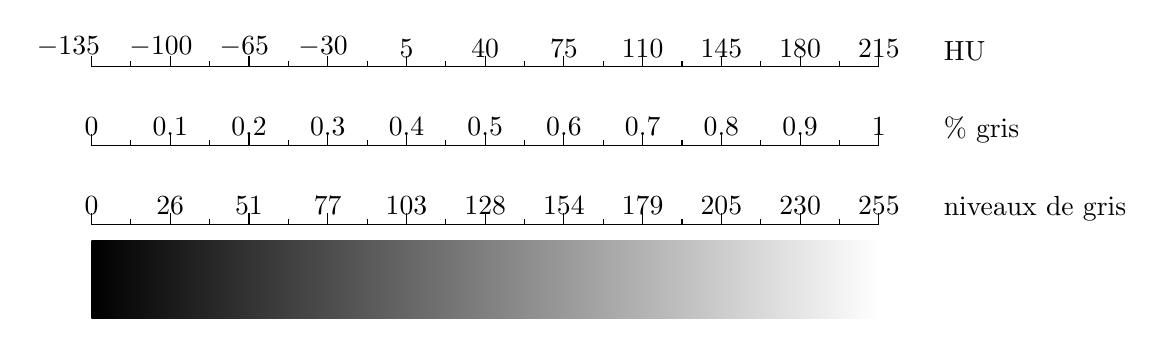
\begin{tikzpicture}
  \shade[left color=black, right color=white] (0,0) rectangle (10,1);   
  \draw (0,1.2) -- (10,1.2) ;
  \draw (0,2.2) -- (10,2.2) ;
  \draw (0,3.2) -- (10,3.2) ;
  \foreach \x/\xtexta/\xtextb/\xtextc in {0/0/0/-135\ \ \ \ \  ,
  1/0.1/26/-100\ \ , %%%pour forcer des espaces
  2/0.2/51/-65\ , 
  3/0.3/77/-30\ , 
  4/0.4/103/5, 
  5/0.5/128/40, 
  6/0.6/154/75, 
  7/0.7/179/110, 
  8/0.8/205/145, 
  9/0.9/230/180, 
  10/1/255/215}{
    \draw[shift={(\x,1.2)}] (0pt,4pt) -- (0pt,0pt) node[above] {$\xtextb$};    
    \draw[shift={(\x,2.2)}] (0pt,4pt) -- (0pt,0pt) node[above] {$\xtexta$};
    \draw[shift={(\x,3.2)}] (0pt,4pt) -- (0pt,0pt) node[above] {$\xtextc$};
    }
  \foreach \x in {0,1,2,3,4,5,6,7,8,9}{
  	\draw[shift={(\x+0.5,1.2)}] (0pt,2pt) -- (0pt,0pt) ; 
  	\draw[shift={(\x+0.5,2.2)}] (0pt,2pt) -- (0pt,0pt) ;
  	\draw[shift={(\x+0.5,3.2)}] (0pt,2pt) -- (0pt,0pt) ;
  	}
  	\draw (10.7,3.4) node[right] {HU};   
  	\draw (10.7,2.4) node[right] { \% gris}; 
  	\draw (10.7,1.4) node[right] {niveaux de gris};     
\end{tikzpicture}
\caption{\label{fig:schema_correspondance_gris} Correspondance des niveaux de gris }
\end{figure}
\todo[noline]{Titre figure \ref{fig:schema_correspondance_gris} à revoir ...}